\chapter{Introduction}
\label{chap:introduction}


Maps are the main tool to represent geographical information. 
As geographical information is usually scale-dependent
\parencite{Muller1995Generalization,Weibel1997}, 
users need to have access to maps at different scales.
In order to generate these maps,
national mapping agencies produce a base map
and then derive maps at smaller scales by 
\emph{map generalization}
More specifically, map generalization is 
the process of extracting and rearranging 
the geographical information of a larger-scale map 
in order to produce smaller-scale maps.
A requirement of map generalization is to emphasize the 
essential while suppress the unimportant,
and at the same time maintain logical relationship between 
objects \parencite{Weibel1997}.
As manual generalization is labor-intensive
\parencite{Duchene2014},
automating map generalization is a promising way 
to produce up-to-date maps at high speed and low cost 
\parencite{Mackaness2017Generalization}.


In our digital age, people interactively read maps 
on computers and mobile phones.
An often used interaction is zooming. 
When users zoom in or out, 
a map must be changed to provide information 
appropriate to the corresponding zoom level.
However, large discrete changes may distract users.
The \emph{on-the-fly generalization}~\parencite{Weibel2017Fly},
which generalizes features in real time, can mitigate this problem.
Still, large discrete changes can be introduced.
By a usability test, \textcite{Midtbo2007} have shown that 
a map is easier to follow 
if the map extent transits smoothly than stepwise. 
In addition to smoothly transiting map extent, 
we want to change also map features smoothly 
when users are zooming.
we believe that this strategy will allow users 
to follow maps even more easily.
The process of producing maps at any different scales
with smooth changes 
is known as \emph{continuous map generalization} (CMG), 
or simply \emph{continuous generalization}.
Ideally, there should be no discrete change in CMG.
However, the term is also used when 
the discrete changes are small enough not to be noticed as,
e.g., \textcite{Suba2016Road} state.



\section{State of the Art}
\label{sec:Intro_State}


CMG has received a lot of attention
from cartographers and computer scientists.
\Textcite{vanKreveld2001} proposed five gradual changes
to support the continuous zooming of maps, 
which are \emph{moving}, \emph{rotating}, \emph{morphing}, 
\emph{fading}, and \emph{appearing}. 
He suggested using these gradual changes 
to adapt discrete generalization operators for CMG.
\textcite{Sester2005_CG} suggested simplifying building
footprints based on small incremental steps and 
to animate each step smoothly.
\textcite{Li2012Continuous} built hierarchies of road segments,
which they then used to omit road segments 
from lower levels of the hierarchy.
Moreover, they evaluated similarities 
between their results and existing maps.
%\textcite{Peng2017Building} gradually grew
%buildings to built-up areas by aggregating buildings 
%whenever they become too close.
\textcite{Touya2017Progressive} progressively replaced
buildings with blocks. 
In addition, their method automatically inferred landmarks 
and put the landmarks on top of the blocks.
\textcite{Suba2016Road} continuously generalized road networks
which are represented as a set of areas.
Their method repeatedly finds the least-important area 
and then either merges it with an adjacent area 
or collapses it to a line segment.
\textcite{Danciger2009} investigated the growing of regions, 
while preserving topology, area ratios, and
relative positions.
The strategy of using two maps at different scales
to generate intermediate-scale maps has been studied in multiple
representations, e.g., with respect to the selection of roads or
rivers~\parencite{Peng2012River,Girres2014}. 
Actually, this strategy is the key idea of the
morphing-based methods for CMG.
In order to morph from one polyline to another polyline,
which respectively represent, say, roads on a larger-scale map 
and a smaller-scale map, we first need to compute 
corresponding points between them 
\parencite[e.g.,][]{Cecconi2003,Noellenburg2008,Chazal2010BallMap,
Deng2015,Li2017_Building,Li2017Annealing}.
Then morphing can be realized by interpolating a set of 
intermediate polylines.
% Among the methods of computing corresponding points,
\textcite{Noellenburg2008} computed an optimum
correspondence between two given polylines 
according to some cost function.
While straight-line trajectories 
are often used for interpolation
\parencite[e.g.,][]{Cecconi2003,Deng2015},
\textcite{Whited2011BallMorph} considered four other alternatives, 
i.e., \emph{hat}, \emph{tangent}, \emph{circular}, 
and \emph{parabolic} paths
based on so-called \emph{ball-map}
\parencite{Chazal2010BallMap}.
%\textcite{Peng2013LSA} defined trajectories requiring that
%angles in vertices and edge lengths should change linearly.
%As these requirements may not agree with each other,
%their method mediates between them using 
%least-squares adjustments.
%\textcite{Peng2016Admin} morphed county boundaries
%to provincial boundaries.
%For county boundaries that do not have corresponding 
%provincial boundaries, they generated the correspondences based 
%on \emph{compatible triangulations}.
\Textcite{vanOosterom2014tGAP} used
a data structure called
\emph{smooth topological generalized area partitioning}
to support visualizing CMG.
One of their contributions is that
a polygon is merged into another polygon continuously
by moving the boundary of the former.
\textcite{Huang2017Matrix} proposed a matrix-based structure 
to support CMG,
using a river network as an example.
For a given scale, 
their structure yields the rivers that should be kept 
as well as how much these rivers should be simplified.



\mypar{Optimization in map generalization}
Map generalization generally specifies 
and takes into account requirements
in order to produce maps of high quality
\parencite{Stoter2009Requirements}.
We categorize requirements as hard and soft constraints.
For example, when users zoom out, 
some land-cover areas become too small to be seen.
These areas need to be aggregated.
When we aggregate one area into another, 
the type of the former is changed to the type of the latter. 
In this problem, a hard constraint could be that 
we aggregate only two polygons at each step 
in order to keep changes small
(see for example \fig\ref{fig:Intro_SubdivisionName}). 
A soft constraint could be that 
we wish to minimize the changes of types, e.g., 
we prefer aggregating a grass area into a farm area 
rather than into a settlement area.
This is a typical \emph{optimization} problem,
where we stick to hard constraints and 
try to fulfill soft ones as good as possible.
Optimization for map generalization is important 
not only because it finds optimal solutions,
but also because it helps us to evaluate the quality of a model
\parencite{Haunert2017Label,
Haunert2008Assuring,Haunert2016Optimization}.
Recall that we wish to minimize the changes of types
when aggregating areas one by one.
A model could be to minimize 
the \emph{smallest} change over all the steps.
Using optimization, we are able to find optimal solutions
of this model at least for small instances.
If even the optimal solutions are bad,
then the model is not reasonable.
In this case, we should improve the model; 
we may want to minimize 
the \emph{average} change over all the steps.
Moreover, optimization is useful for evaluating heuristics.
We need heuristics because
many optimization problems cannot be solved efficiently
\parencite[e.g.,][]{HaunertWolff2010AreaAgg,Haunert2016Partition}.
While heuristics can find some solutions in reasonable time,
it is important to know the quality of 
these solutions.
Fortunately, we can often find an optimal solution when 
the size of an instance is sufficiently small.
Consequently, we are able to evaluate 
the quality of a heuristic 
by comparing its results with optimal solutions
on small instances.

%\todo{may cite \textcite{Bader2001Dissertation}}

\begin{figure}[tb]
\centering
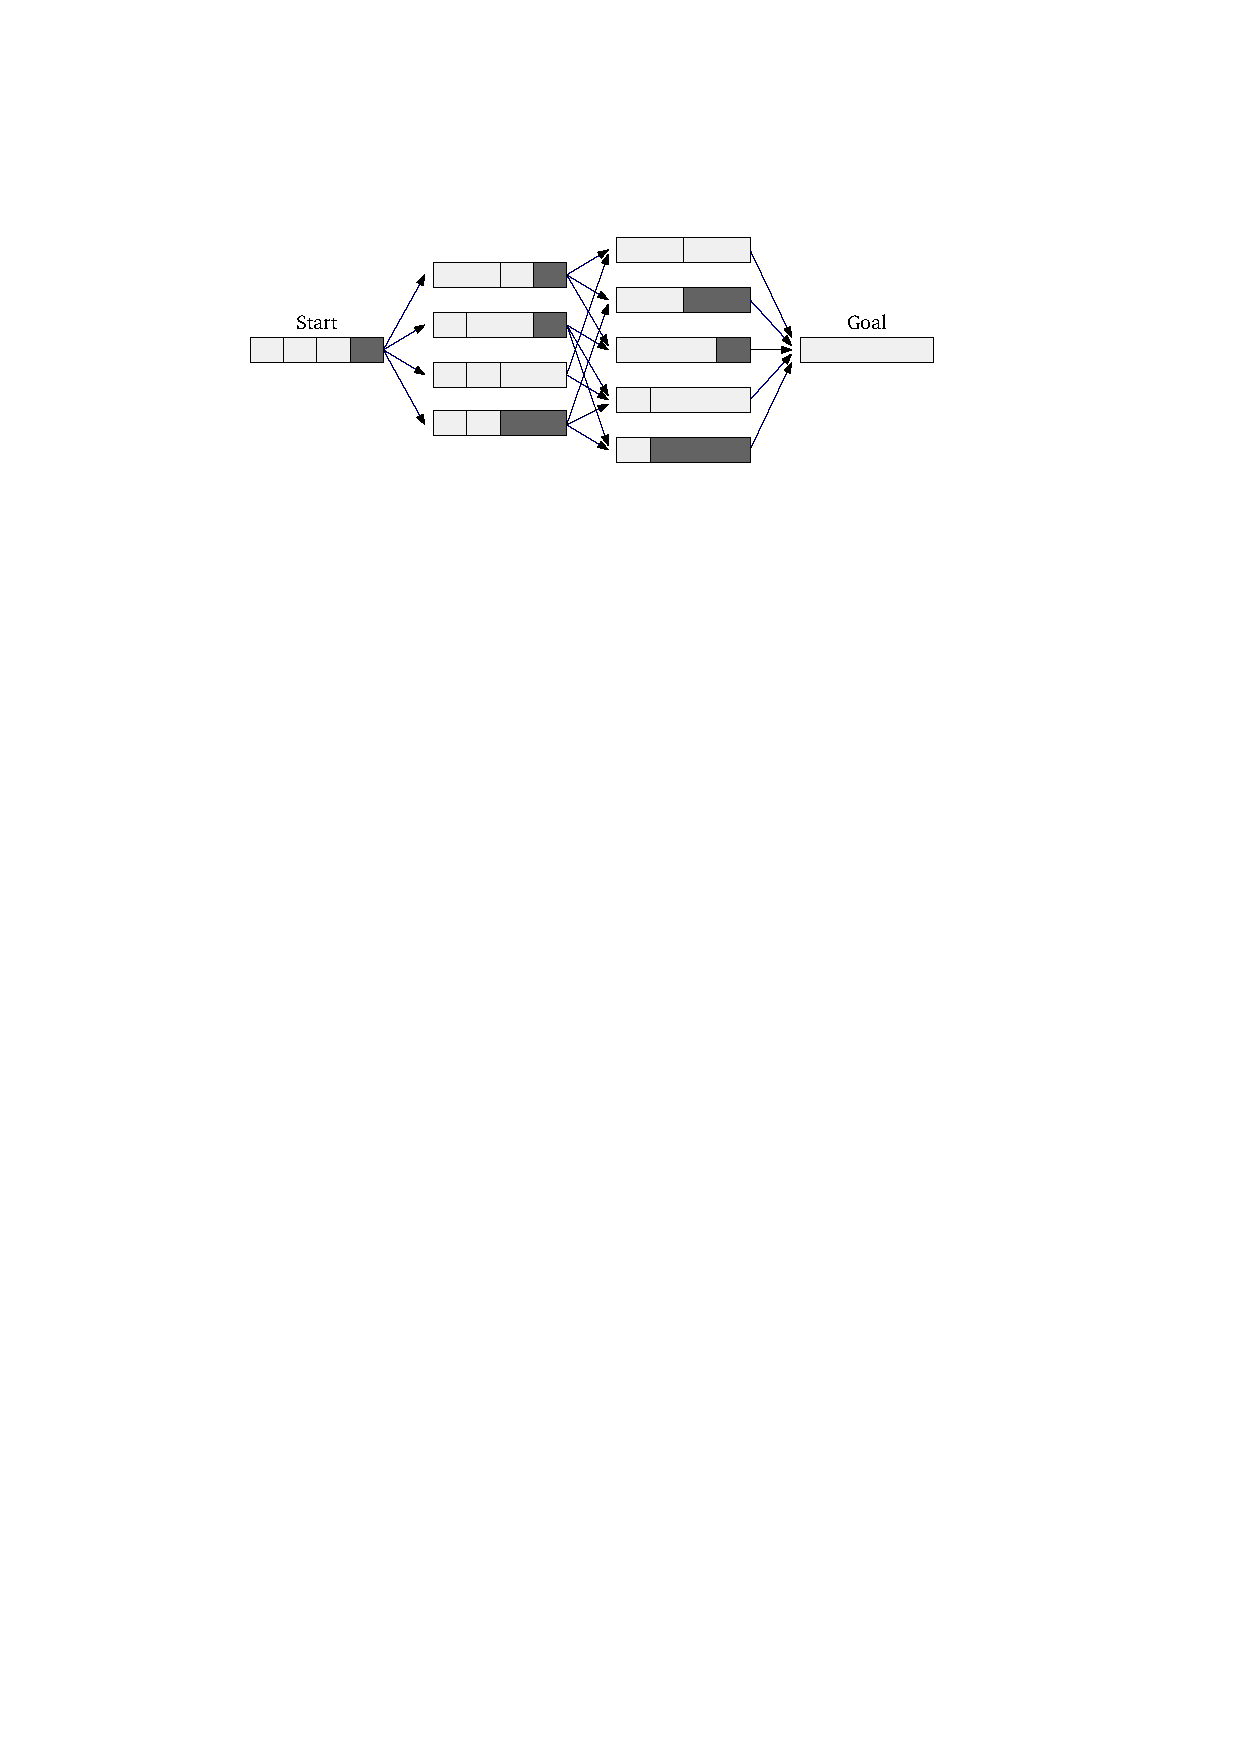
\includegraphics[page=1]{Intro}
\caption{There are many ways of aggregating a set of land 
cover areas to a single one.}
\label{fig:Intro_SubdivisionName}
\end{figure}

Optimization has been widely used in map generalization.
For example, \textcite{Harrie1999} displaced objects 
based on least-squares adjustments (LSA)
to solve spatial conflicts.
In his problem, the soft constraints 
for shapes and locations may contradict each other.
Therefore, it is necessary 
to mediate between these constraints, 
which can be done by LSA.
\textcite{Sester2005Optimization} used LSA not only for 
displacing objects but also for simplifying buildings. 
She required that 
the output boundaries should be 
as close to the original buildings as possible.
\textcite{Tong2015AreaLSA} generalized land-cover areas,
where LSA was used to preserve the sizes of 
the land-cover areas.
\textcite{Regnauld2001} grouped buildings based on 
minimum spanning trees in order to typify
the buildings in a group.
\textcite{Burghardt2005Snakes} smoothed lines based on 
energy minimization. 
According to his setting, a line contains less energy
if it is smooth and close to the original line.
He repeatedly displaced the line 
until finding a stable state 
in terms of minimizing his energy function.
\textcite{HaunertWolff2010AreaAgg} aggregated land-cover areas
based on mixed-integer linear programming.
This method is based on global optimization and minimizes 
type changes as well as a cost for non-compact shapes 
while satisfying constraints on the sizes of the output regions.
\textcite{Haunertwolff2010Building} simplified building
footprints by solving an integer linear program (ILP).
They aimed at minimizing the number of edges in the output 
under the restriction that 
the simplified buildings must be topologically safe,
that is, the selected and extended edges must not intersect with 
each other.
\textcite{Oehrlein2017Aggregation} aggregated the departments 
of France according to unemployment rates based on integer 
linear programming; they used a cutting-plane method to 
speed up solving their ILP.
\textcite{Funke2017Simplification} simplified 
administrative boundaries based on an ILP.
Their aim was to minimize the number of edges
while keeping the result boundaries close to the original ones
and avoiding any intersection. 
At the same time, the required that every city, 
represented by a point, 
stays in the same face as before the generalization.



\mypar{Optimization in \emph{continuous} map generalization}
Optimization becomes more delicate
when we deal with CMG.
In this field, we have requirements 
not only for a specific map, 
but also for relations between maps. 
%
Nevertheless, some optimization techniques 
have been applied to CMG.
In the aforementioned article,
\textcite{Noellenburg2008} used dynamic programming
to match points of two polylines to support morphing
according to some matching cost.
\textcite{sahw-oarps-ICAGW13} used 
mixed-integer linear programming 
to select points of interest.
They required that 
a point, once disappeared, should not show up again 
during zooming out. 
They also required that any two points should be 
sufficiently far away from each other.
Based on these requirements, 
they wanted to show as many points as possible 
for a given scale interval.
\textcite{Chimani2014Eat} computed a deletion sequence
for a road network by integer linear programming
and efficient approximation algorithms.
They wanted to delete a stroke, 
which is a sequence of edges, at each step
while keeping the remaining network connected.
They assigned each edge a weight, 
and their objective was to maximize the total weight 
over all the road networks of all the steps.
%\textcite{Peng2013LSA} defined trajectories 
%based on LSA for morphing between polylines, 
%where LSA is used to mediate between the requirements 
%for angles and edge lengths of the intermediate polylines.

\section{Tools for Optimization}
\label{sec:Intro_Tools}

In this thesis, we use some well-known optimization methods,
namely, the \Astar algorithm \parencite{Hart1968}, 
integer linear programming
\parencite[chapter~13]{Papadimitriou1982combinatorial},
dynamic programing \parencite[chapter~15]{Cormen2009}, and
least-squares adjustment (LSA) \parencite[chapter~3]{Koch1988}.
We also use the minimum spanning tree;
see \textcite[chapter~23]{Cormen2009}.
%
We use \Astar and integer linear programming 
to find optimal sequences for 
area aggregation (see \chap\ref{chap:AreaAgg}).
Similar to \textcite{Noellenburg2008},
we use dynamic programming to 
compute corresponding points between polylines
(see \chaps\ref{chap:Admin} and \ref{chap:Morph}).
We use the minimum spanning tree to group buildings,
which is similar to \textcite{Regnauld2001}; 
see \chap\ref{chap:Bldg}.
We define trajectories based on LSA 
for morphing between polylines (see \chap\ref{chap:Morph}).
% There is no optimization used in \chap\ref{chap:DataStr}.
In the following, we briefly recall these methods.


Given a graph with nodes and weighted edges,
a typical task is to find a shortest path 
from a start node to a goal node.
A breadth-first search \parencite[chapter~22]{Cormen2009}
solves the shortest-path problem 
in unweighted graphs.
Dijkstra's algorithm \parencite{Dijkstra1959}
always chooses from the explored nodes the neighbor 
with minimum distance from the start node. 
The \Astar algorithm is 
a generalized version of Dijkstra's algorithm.
When \Astar chooses a node to explore the neighbors,
the algorithm does not only take into account 
the distance from the start node
but also estimates the distance to the goal node.
By always choosing a node which is likely 
to be closer to the goal node, 
\Astar often explores fewer nodes than Dijkstra's algorithm
in finding a shortest path.
If the estimated distances are always smaller than the exact 
distances to the goal node, 
then \Astar will find a shortest path.

Linear programming models an optimization problem as objective 
functions subject to constraints,
where the objective functions and constraints are represented by 
linear functions of some variables.
These constraints form a convex polyhedron.
An optimal solution lies on the boundary of the polyhedron and 
can be found efficiently.
\emph{Integer} linear programming requires that
the variables must use integers.
Integer linear programming is NP-hard
since many NP-hard problems such as vertex cover can be 
formulated as integer linear programs.
Intuitively, this is due to the fact that the optimal solution 
may lie in the interior of the polyhedron, where geometry does 
not help to find it.
If only some of the variables are required to be integers
(other variables are allowed to be non-integers), 
then the problem is called mixed integer linear programming,
which is also known as NP-hard; see for more details
\textcite[chapter~16]{Schrijver1986}.



Dynamic programming decomposes 
a big instance of a complex problem 
into a collection of smaller subinstances.
The method solves each subinstance just once 
and saves the solution. 
The next time when the same subinstance occurs, 
the method will use the previously computed solution 
instead of resolving this subinstance. 
In this way, the method saves computation time.
Other than in the divide-and-conquer approach used, 
e.g., in Mergesort, 
in dynamic programming subinstances of equal size 
are usually \emph{not} disjoint but overlap.

Least-squares adjustment is a model for solving 
over-constrained problems.  
It handles computes a set of unknowns 
based on a set of observations.
Because of errors, the observations may contradict each other.
We have to adjust the observations 
so that we can obtain a set of unknowns that agree 
all the adjusted observations.
There can be infinitely many sets of adjustments feasible, 
but we choose the one with the least sum of squared adjustments.
Based on this set of adjustments,
we can finally compute the unknowns.


Given a graph with nodes and weighted edges, 
a minimum spanning tree (MST) of the graph 
is a minimum-weight subset
of the edges that together connect all nodes.
Surprisingly, the MST can be computed 
by simple greedy algorithms
such as Kruskal's algorithm \parencite{Kruskal1956}
or the algorithm of Jarn\'ik--Prim 
\parencite{Jarnik1930,Prim1957}.
Strictly speaking, the MST by itself is not 
an optimization \emph{method}, 
but it is a helpful structure of low weight 
that helps to solve many optimization problems 
in graph theory at least approximately, 
for example, the metric version of the famous Traveling
Salesperson Problem (TSP).


\section{Overview of the Thesis}
\label{sec:Intro_Overview}

This thesis contains five chapters 
that deal with methods for continuous map generalization. 
First, we find optimal sequences 
for aggregating land-cover areas.
%
Second, we continuously generalize county boundaries to
provincial boundaries.
%
Third, we continuously generalize buildings to built-up areas 
by aggregating and growing.
%
Fourth, we define moving trajectories
based on least-squares adjustment
for morphing between polylines.
%
Fifth, we discuss the performance 
of data structures for spatial problems.
%
In the remainder of this section, 
we present our results in more detail.


\subsubsection{%
Finding Optimal Sequences for Area Aggregation---\\
\Astar vs. Integer Linear Programming}

To provide users with maps of different scales and 
to allow them to zoom in and out without losing context,
automatic methods for map generalization are needed.
We approach this problem for land-cover maps.
%Given two maps of the same region at two different scales,
%a relevant problem is to compute maps for any intermediate scale.
Given two land-cover maps at two different scales, 
we want to find a sequence of small incremental
% To help map users not to lose context during zooming,
% we try to provide maps that change as continuous as possible.
% Since maps at some different scales often exist, 
% a relevant problem is to find maps at any intermediate scales.
% Given two land-cover maps of different scales, 
% we wish to find a sequence of small incremental
changes that gradually transforms one map into the other.
We assume that the two input maps consist of polygons 
each of which belongs to a given land-cover class. 
Every polygon on the smaller-scale map
is the union of a set of adjacent polygons 
on the larger-scale map. 

In each step of the sequence that we compute, 
the smallest area is merged with one of its neighbors. 
We do not select that neighbor according to a prescribed rule 
but compute the whole sequence of pairwise merges at once, 
based on global optimization.
We formalize this optimization problem as that of 
finding a shortest path in a (very large) graph.
%We compared the \Astar algorithm and 
%integer linear programming in solving this problem.
For solving such a problem, standard approaches
are the \Astar algorithm or integer linear programming.
%We compare how the two methods solve our problem.
To avoid long computing times, we allow the two methods to 
return non-optimal results.
In addition, we present a greedy algorithm 
as a benchmark.
We tested the three methods with a
dataset of the official German topographic database ATKIS.
Our main result is that
\Astar finds optimal aggregation sequences for more instances 
than the other two methods
within a given time frame.
\fig\ref{fig:Intro_AreaAgg_Case612} shows some intermediate 
results obtained by \Astar for one of the regions.
This is joint work with Alexander Wolff and Jan-Hendrik Haunert,
part of which has been published~\parencite[see][]{Peng2017AStar}.


\begin{figure}[tb]
\centering
\includegraphics[page=2]{Intro}
\caption{Some intermediate aggregation results of 
	a region (Buchholz in der Nordheide, Germany). 
	There are $9$ polygons on 
	the larger-scale map (top left). 
	These areas are aggregated into one 
	on the smaller-scale map (bottom left). 
	The digits are the numbers of the areas.
}
\label{fig:Intro_AreaAgg_Case612}
\end{figure}

\subsubsection{%
Continuously Generalizing Administrative Boundaries\\
Based on Compatible Triangulations}

Topological consistency is a key issue 
in cartographic generalization.
Our aim in this chapter is to ensure topological consistency  
during continuous map generalization 
of administrative boundaries.
To this end, we present a five-step method.
Our inputs are two maps of administrative boundaries 
at different scales, 
where the larger-scale map has not only more details 
but also an additional level of administrative regions.

Our main contribution is the proposal of a workflow for
generalizing hierarchical administrative boundaries in a
continuous and topologically consistent way.  First, we
identify corresponding boundaries between the two maps.
We call the remaining boundary pieces (on the larger-scale map)
\emph{unmatched} boundaries.  
Second, for the unmatched boundaries,
we generate their corresponding boundaries 
on the smaller-scale map
based on compatible triangulations. 
Third, we simplify the generated boundaries
by Douglas--Peukcer algorithm.  
Fourth, we compute corresponding points for each pair
of corresponding boundaries using a variant of an existing 
dynamic programming algorithm.  
Fifth, we interpolate between the corresponding points
to generate the boundaries at intermediate scales.

We do a thorough case study 
on the provincial and the county boundaries of Mainland China.
Although topologically consistent algorithms 
for the third step and the fifth step exist, 
we have implemented simpler algorithms for our case study. 
\fig\ref{fig:Intro_AdminBound_Tianjin} shows our results of 
continuously generalizing county boundaries 
to provincial boundaries of Tianjin, China.
This is joint work with Alexander Wolff 
and Jan-Hendrik Haunert~\parencite[see][]{Peng2016Admin}.

\begin{figure}[tb]
\centering
\includegraphics[page=3]{Intro}
\caption{Continuously generalizing county boundaries to 
provincial boundaries of Tianjin province, China.}
\label{fig:Intro_AdminBound_Tianjin}
\end{figure}

\subsubsection{%
Continuously Generalizing Buildings to Built-up Areas\\
by Aggregating and Growing}

To enable smooth zooming, 
we propose a method to continuously generalize buildings 
from a given start map to a smaller-scale goal map, 
where there are only built-up area polygons 
instead of individual building polygons
(see Figure~\ref{fig:Intro_BldgGrow}).
We name the buildings on the start map 
\emph{original buildings}.
%
For an intermediate scale, 
we aggregate the original buildings that will become too close 
by adding bridges.
We grow the (bridged) original buildings based on buffering 
and simplify the grown buildings.
We take into account the shapes of the buildings 
on both the preceding map and the goal map to make sure that 
the buildings are always growing.
The running time of our method is in~$O(n^3)$,
where~$n$ is the total number of edges
overall the original buildings.
%

The advantages of our method are as follows. 
First, we grow the buildings continuously 
and, at the same time, simplify the grown buildings.
Second, right angles of buildings are preserved during growing: 
the merged buildings still look like buildings. 
Third, the distances between buildings are 
always larger than a specified threshold.
We do a case study to show the performances of our method.
This is joint work with 
Guillaume Touya~\parencite[see][]{Peng2017Building}.

\begin{figure}[tb]
\centering
%\includegraphics[page=4]{Intro}
\includegraphics[page=4]{Bldg_CaseStudy_DataAndResults}
\caption{Continuously generalizing buildings to built-up 
	areas by aggregating and growing.}
\label{fig:Intro_BldgGrow}
\end{figure}


\subsubsection{Morphing Polylines 
	Based on Least-Squares Adjustment}

One way of continuously generalizing polylines 
is to use morphing techniques. 
Most often for morphing, 
the vertices of the polylines move on 
defined straight-line trajectories at constant speeds.
In this chapter we address morphing of polylines, 
but we relax the requirement that 
the vertices of the polylines move on straight lines. 
Our concern with straight-line trajectories is that 
characteristic properties (e.g., bends) of the polylines 
change drastically during the morphing process. 
In particular, we suggest that 
the angles and the edge lengths of the polylines 
should change linearly during the morphing process. 
This expectation is clearly not accomplished 
with straight-line trajectories. 
In contrast, we present a new method 
based on least-squares adjustment 
that yields close-to-linear changes of 
the angles and the edge lengths. 
Figure~\ref{fig:Intro_LSA_Compare} 
shows a comparison of morphing based on 
straight-line trajectories and our new morphing method.
This is joint work 
with Jan-Henrik Haunert, Alexander Wolff, 
and Christophe Hurter~\parencite[see][]{Peng2013LSA}.

\begin{figure}[htb]
\centering
\includegraphics[page=2]{Morph_CaseStudy_Artificial}
\caption{A comparison of morphing 
    based on the two different trajectories.}
\label{fig:Intro_LSA_Compare}
\end{figure}

\subsubsection{Choosing the Right Data Structures 
	for Solving Spatial Problems}

When we plan to implement a program, 
there are always many data structures that
we can use to achieve a certain goal.
However, if we do not carefully choose and use 
the data structures,
the implemented program may be inefficient.
As an example, we consider the problem of 
finding pairs of close points from a dataset. 
We consider two points to be close 
if they lie within a square of pre-specified 
side length~$\varepsilon$. 
We compare three obvious algorithms to solve the problem: 
a sweep-line (SL) algorithm, 
an algorithm based on the Delaunay triangulation (DT) 
of the input points, 
and a hashing-like algorithm 
which overlays the input points with a rectangular grid. 
We implemented the algorithms in C\# and tested them on 
randomly generated data and real-world data. 
We used the DT available in ArcGIS Objects. 
We used three different data structures
of \emph{balanced binary search} tree, 
i.e., SortedDictionary (SD), SortedSet (SS), and TreeSet (TS), 
to implement the sweep-line algorithm. 
The simple grid-based algorithm turned out to run faster than 
any of the other algorithms by a factor of at least~$2$ 
(see Figure~\ref{fig:Intro_DataStructure}).
This is joint work with 
Alexander Wolff~\parencite[see][]{Peng2014DataStr}.

%\bigskip
%The thesis is closed with a summary and a list of open problems.

\begin{figure}[tb]
\centering

\includegraphics[page=2]{DataStr_Plot_Bavaria}
\caption{Time consumption of the algorithms
	for computing close point pairs. 
	Two points are defined as close if the differences 
	of their $x$- and $y$- coordinates are both smaller than
	$\varepsilon=0.001267 \degree$,
	where the coordinates are with unit degree. 
	The DT-based algorithm took $262\,$s 
	with radius $r_1=\varepsilon \cdot (1+\sqrt{2})/2$ 
	("DT $r_1$") and $784\,$s 
	with radius $r_2=\varepsilon \cdot (1+\sqrt{7})/2$ 
	("DT $r_2$") for $n=553{,}984$ points.
	The curve labeled "DT constr." represents 
	the time for constructing 
	Delaunay triangulations for the input points.
}
\label{fig:Intro_DataStructure}
\end{figure}


{\setlength{\parskip}{0ex}

\section{Acknowledgments}

Obtaining a PhD in Germany was 
one of the best things I could dream of.
When I finally got the chance to study in Germany,
I was thrilled and I wanted to do my best.
Now I feel so proud of myself because I have come this far.
Of course, this thesis would not have been possible
if it was not for the help of many people.

First of all, I would like to thank my supervisor, 
Prof.\ Dr.\ Alexander ``Sascha'' Wolff.
I~am grateful to him for giving me 
the opportunity to pursue my PhD in his group.
The research work was challenging,
but I enjoyed working with him.
Sascha has been very patient with me.
When I first came to Germany, I could barely speak English.
He had to put a lot of effort into understanding me
when we were doing research.
Sascha advised me to take lectures and sent me to conferences
so that I could learn as much as possible.
Sascha always encouraged me to ask questions
because I can benefit from the answers.
He told me not to be shy even when 
I fear that the questions are stupid;
other people in the audience may appreciate my asking
because they may have the same questions,
but don't dare to ask.
%% Here, the point is not so clear (and not so exciting); I'd drop it.
% Sascha always responded my requests promptly.
% Once, I noticed that I was missing a letter from him 
% for some business on the next day
% while he was attending a conference in Italy.
% Nevertheless, after I had written him an email,
% he sent me the letter before 20:00.
At some point,
Sascha even negotiated with my landlords 
when I moved from an apartment into another.
Moreover, Sascha has a good sense of humor, 
and we often cracked jokes together.
I was lucky to have him as my supervisor.

I also thank my second supervisor, 
Prof.\ Dr.\ Jan-Henrik Haunert.  
In his lecture \emph{Algorithms for GIS}, 
he taught me many fundamentals of GIScience.  
Later, he moved to other universities 
and invited me to visit him there.
During the visits, we sketched many ideas together.
In particular, he proposed % the research of 
using the \Astar algorithm 
for finding optimal sequences for area aggregation,
which led to the most important chapter of my thesis.
Furthermore, he recommended many suitable conferences to me
when I wanted to publish my papers.
% He taught me the ``optimization mantra'' (explain?).
% DP: I do not understand ``optimization mantra''
% AW: A "mantra" is a sequence of words that are repeated over and
% over because they are so important:
% https://en.wikipedia.org/wiki/Mantra
% Mantras [....] helps to induce an altered state of consciousness.
% :-)

I am grateful to all the colleagues in our group:
Moritz Beck, Johannes Blum, Benedikt Budig, 
Steven Chaplick, Thomas van Dijk, 
Martin Fink, Oksana Firman, Krzysztof Fleszar, 
Philipp Kindermann, Myroslav Kryven, 
Fabian Lipp, Andre L\"offler, 
Nadine Schwartges, Joachim Spoerhase, Sabine Storandt, 
and Johannes Zink.
%
We often had coffees together,
and it was a lot of fun to play squash and to go out for our excursions.
It was nice that our group always had lunch together
so that we had plenty of chances to learn from each other.
Indeed, I sometimes took advantage of these lunches
to get suggestions regarding my research work.

I am indebted to Dr.\ Krzysztof Fleszar for 
helping me a lot during my PhD study.
He is very warm-hearted.
Whenever he found that I had problems to understand a paper,
he read that paper and then explained it to me.
He always helped when I needed a German--English translator.
He helped me move twice using the van of his family.
On the day before my defense, he worked as hard as me
to read my slides and to give me feedback.
He has always invited me to join his parties, 
and I am grateful to him for his invitations.

I thank Dr.\ Guillaume Touya for inviting me to visit
the French National Mapping Agency (IGN).
The visit was a great chance and gave me insight into
practical requirements regarding maps.
Our collaboration resulted in a paper on continuously
generalizing buildings into built-up areas.
%
I also thank Dr.\ Thomas van Dijk.
He helped me speed up my 
least-squares adjustment using a C++ library.
He has proofread some of my papers
and has given me helpful suggestions 
concerning many aspects of my research.

I am grateful to Prof.\ Dr.\ Min Deng.
He introduced me into the research area of 
continuous map generalization 
and helped me to get the chance of
pursuing my PhD at the University of W\"urzburg.

I thank Prof.\ Dr.\ Dirk Burghardt 
for quickly reviewing my thesis
when my working contract in W\"urzburg was about to end.
I also thank him for introducing my research work to
Prof.\ Dr.\ Peter van Oosterom, 
which certainly helped me to get a postdoc position
in Peter's group.
Before submitting the final version of my PhD thesis,
I have been working in Peter's group.
I would like to thank 
Prof.\ Dr.\ Peter van Oosterom and Dr.\ Martijn Meijers 
for allowing me to finish my paper about area aggregation,
which is part of this thesis. 
I thank Prof.\ Dr.\ Andreas N\"uchter for chairing my defense.

I would like to thank my parents
for all their love and encouragement.
I thank them for their suggestions 
when I was making decisions.
My special thanks go to Fang Wu.
She has been very supportive of me.
We enjoyed many activities together, 
including hiking, skating, skiing, shopping, and so on.
She made my life much more colorful.

I thank all my friends in W\"urzburg
for their company.

Last but not least, 
I am very grateful to the University of W\"urzburg 
because I had the possibility take many courses.
In order to gain sufficient credits for 
obtaining my Ph.D.\ degree in Computer Science,
I took some courses
(e.g., \emph{Theoretical Computer Science}
and \emph{Algorithms and Data Structures})
in my own faculty, 
the Faculty of Mathematics and Computer Science.
%
In order to improve my language skills,
I took many courses
offered by the Language Center
(e.g., \emph{English for the Natural Sciences} 
and \emph{General Language Exercise of German})
and by the Faculty of Arts 
(e.g., \emph{Introduction to English Linguistics}).

}